\documentclass[article,nojss]{jss}

\usepackage{listings}
\usepackage{hyperref}

\DeclareGraphicsExtensions{.pdf,.eps}
\newcommand{\fct}[1]{{\code{#1()}}}
\newcommand{\class}[1]{{`\code{#1}'}}


\author{Marco Smolla \And Bart Kranstauber}
\Plainauthor{Marco Smolla, Bart Kranstauber}

\title{An introduction to the 'move' package}
\Plaintitle{Using the move package}

\Keywords{animal track, time series, utilization density, gps}

\Abstract{
  The move package provides a series of functions to import, visualize and analyze animal movement related data in an object-oriented way. The introduced classes allow one to store data that are related to an individual in one object, such as coordinates and timestamps, name, species, age, sex, study site, etc. This makes working with multiple animals, or multiple seasons much easier. Furthermore, the package includes functions to calculate home ranges (Minimum Convex Polygon Bootstrap) and utilization distributions (UDs). The latter uses the dynamic Brownian Bridge Movement Model to calculate animal UDs.\\
}

\Address{
  Marco Smolla\\
  Max-Planck-Institute for Ornithology, Radolfzell, Germany\\
  E-mail: \email{msmolla@orn.mpg.de}\\

  Bart Kranstauber\\
  Max-Planck-Institute for Ornithology, Radolfzell, Germany\\
  E-mail: \email{kranstauber@orn.mpg.de}\\
}

\usepackage{Sweave}
\begin{document}
\input{move-concordance}


%\VignetteIndexEntry{How to use the move package}
%\VignetteDepends{sp, raster, rgdal, methods, geosphere}
%\VignetteKeywords{GPS, time series, track}
%\VignettePackage{move}


\section*{Introduction}
The amount of recorded animal movement data is increasing. The data offer information about land use, animal distribution, interactions between the environment and much more. The enormous amount of data needs to be analyzed with mathematical algorithms. The programming language R, developed by the R Development Core Team, offers an easy to learn environment to do statistical analyses. It even supports object-oriented programming. The package we present here offers additional functions that are specially made to analyze animal movement data. \\
Movement data that are associated with individual animals or a group of animals can be imported into R and stored as a single object. These objects can include all kinds of information. The minimum requirement however are timestamps, coordinates, and a unique ID per animal. Further attributes of the objects can be sensor types, body size, sex, weight, etc. \\
A lot of data sets are available on a database called Movebank (\url{www.movebank.org}). If a user has the permission to see a data set, one can download it as a .csv (comma separated values) file. Files from Movebank can be directly imported into R. \\
A more recent update of the Move package has added a web-interface. Now it is possible to directly download whole data sets from within R. The only requirement is an account on Movebank and the rights to see the data (see the "browsing Movebank" vignette for more information). \\
Besides importing data from Movebank, it is also possible to use personal data sets, as long as they meet the minimum requirements of timestamps, coordinates, and animal IDs. \\
A series of functions allow one to plot, summarize, and analyze the movement data. Individual \class{Move} objects can be stacked to a MoveStack object which includes a series of animals and the additional data that are associated with them. This allows one to work with many animals at the same time. \\
A new feature, called burst, allows one to subset track information. This can be interesting, for example, if a track should be analyzed depending on specific behaviors (migratory, non-migratory, resting behavior). \\
One of the main features of the move package is the calculation of the utilization distribution (UD), a measure to estimate the home range of an animal. In this version of the package, we use the dynamic Brownian Bridge Movement Model (dBBMM) to calculate the UD. The UD can be calculated for individuals or for a group (stack) of individuals. This results in the object types \class{DBBMM} or \class{DBBMMStack}. These objects store all information that are needed to visualize the UD, including the raster it was calculated for, and the values per raster cell.\\
The following sections introduce the different functions we implemented for the \class{Move}, \class{MoveStack}, \class{DBBMM}, and \class{DBBMMStack} objects. We demonstrate how functions can be used to import, analyze, and visualize animal movement data. The aim of this vignette is to enable all users unfamiliar with the package to handle all basic functions.



%%%%%%%%%%%%%%%%%%%%%%%%%%%%%%%%%%%%%%%%%%%%%%%%%%%%%%%
\section{Data import}
The import of data into R can happen in two ways: either by importing .csv data files (using the \fct{move} function) or by using the web interface of the move package (using the \fct{getMovebankData} function). The web interface allows one to access and download data sets from Movebank. 

\subsection{Import of Movebank data}
Files from Movebank (\url{www.movebank.org}) can be imported with \texttt{move(x="path")}, where "path" is a character string that locates the file on the hard drive. It may look like: \\ \\ \texttt{> data <- move(x="/User/Documents/test.csv")}. \\ \\
The following line imports the "leroy.csv.gz" file that is part of the move package.

\begin{Schunk}
\begin{Sinput}
> leroy <- move(system.file("extdata","leroy.csv.gz",package="move"))
\end{Sinput}
\end{Schunk}

\subsection{Import of non-Movebank data}
If data sets are not published on Movebank but stored on the hard drive they can be imported with the same \fct{move} function. Because the column names may differ from the Movebank standard, it is necessary to indicate the timestamp and coordinates columns, the projection method of the coordinates (e.g. longitude-latitude), and the data frame that includes all of the imported data. The standard \fct{move} method also allows one to directly enter the used sensor type and the animal name. \\
Import of a non-Movebank csv file that is attached to this package:

\begin{Schunk}
\begin{Sinput}
> data <- read.csv(system.file("extdata","ricky.csv.gz",package="move"))
> ricky <- move(x=data$location.long, y=data$location.lat, time=as.POSIXct(data$timestamp, 
+             format="%Y-%m-%d %H:%M:%OS", tz="UTC"), proj=CRS("+proj=longlat"), 
+             data=data, animal=data$individual.local.identifier, sensor=data$sensor)
> ricky 
\end{Sinput}
\begin{Soutput}
class       : Move 
nfeatures   : 8958 
extent      : -73.94032, -73.8683, 42.82073, 42.851  (xmin, xmax, ymin, ymax)
coord. ref. : +proj=longlat +ellps=WGS84 
nvariables  : 18
names       :     X, event.id, eobs.battery.voltage, eobs.fix.battery.voltage, eobs.horizontal.accuracy.estimate, eobs.key.bin.checksum, eobs.speed.accuracy.estimate,    eobs.start.timestamp, eobs.temperature, eobs.used.time.to.get.fix, ground.speed, heading, height.above.ellipsoid, individual.local.identifier, utm.easting, ... 
min values  :     2, 44295482,                 3449,                     3081,                              2.05,                524362,                         0.22, 2010-02-09 17:00:00.000,                0,                         3,         0.00,    0.00,                    0.0,                     Ricky.T,    586587.2, ... 
max values  : 10760, 44529025,                 3740,                     3559,                             95.23,            4294919150,                        48.67, 2010-03-31 17:30:02.000,              -12,                       120,        43.12,  359.79,                 -315.6,                     Ricky.T,    592500.3, ... 
timestamps  : 2010-02-09 17:01:23...2010-03-31 17:31:26 Time difference of 50 days  (start...end, duration) 
sensors     : gps 
indiv. data : behavioural.classification, eobs.status, eobs.type.of.fix, manually.marked.outlier, visible, sensor.type, individual.taxon.canonical.name, tag.local.identifier, study.name, utm.zone, study.timezone 
indiv. value: NA A 3 NA true gps Martes pennanti 1016 Urban fisher GPS tracking 18N Eastern Standard Time 
date created: 2012-12-10 14:13:42 
\end{Soutput}
\end{Schunk}

Entering the object name calls the \fct{show} function of \class{Move} objects. This function provides an overview of the object. It returns the object class (\class{Move}), the animal ID (ricky), number of coordinates (8961), the extent of the coordinates, the coordinates reference system (or projection, here longitude-latitude), the number of columns of the imported data.frame, and the names of the columns of the data.frame, as well as the first and last timestamp and the duration of the observation. The \fct{show} works in a similar way for all other object types.\\


\subsection{Handling multiple animals}
If the data-set includes more than one animal, it is necessary to indicate the column with the animal IDs. The \fct{move} automatically creates a stack of Move objects called \class{MoveStack}. \\
Sometimes it is desirable to work with stacked Move objects. Most functions of the Move package are capable of working with stacks. Stacks are either created when .csv files with multiple animal IDs are imported, or when a \class(list) of \class(Move) objects is passed on to the stacking function \fct{moveStack}.

\begin{Schunk}
\begin{Sinput}
> list <- list(leroy, ricky)
> stack <- moveStack(list)
> stack
\end{Sinput}
\begin{Soutput}
class       : MoveStack 
nfeatures   : 9877 
extent      : -73.94032, -73.84366, 42.70898, 42.851  (xmin, xmax, ymin, ymax)
coord. ref. : +proj=longlat +ellps=WGS84 +datum=WGS84 +towgs84=0,0,0 
nvariables  : 22
names       :           timestamp, eobs.battery.voltage, eobs.horizontal.accuracy.estimate, eobs.key.bin.checksum, eobs.speed.accuracy.estimate,    eobs.start.timestamp, eobs.status, eobs.temperature, eobs.type.of.fix, eobs.used.time.to.get.fix, ground.speed, heading, height.above.ellipsoid, utm.easting, utm.northing, ... 
min values  : 2009-02-11 12:16:45,                 3449,                              2.05,                524362,                         0.22, 2009-02-11 12:14:59.000,           A,                0,                3,                         3,         0.00,    0.00,                    0.0,    586587.2,      4729143, ... 
max values  : 2009-03-04 09:16:59,                 3740,                             97.02,            4294919150,                        48.67, 2010-03-31 17:30:02.000,           A,              -12,                3,                       120,        43.12,  359.79,                 -315.6,    594679.4,      4744839, ... 
timestamps  : 2009-02-11 13:16:45...2010-03-31 19:31:26 Time difference of 413 days  (start...end, duration) 
sensors     : gps 
indiv. data : eobs.fix.battery.voltage, manually.marked.outlier, visible, sensor.type, individual.taxon.canonical.name, tag.local.identifier, individual.local.identifier, study.name, study.timezone, behavioural.classification, eobs.status, eobs.type.of.fix, utm.zone 
min ID Data : NA NA true gps Martes pennanti   74 NA Urban fisher GPS tracking Eastern Standard Time NA NA NA NA 
max ID Data : NA NA true gps Martes pennanti 1016 NA Urban fisher GPS tracking Eastern Standard Time NA NA NA NA 
individuals : Leroy, Ricky.T 
unused rec. : 1071 
date created: 2012-12-10 14:13:42 
\end{Soutput}
\end{Schunk}

The show function works also for the stack object. It combines the information of all objects that are stored in the \class{MoveStack}. \\
It is also possible to break down a \class{MoveStack} into single \class{Move} objects using the \fct{split} function. It returns a list of all \class{Move} objects.


\begin{Schunk}
\begin{Sinput}
> unstacked <- split(stack)
> #use show(unstacked) to see all objects of unstacked
\end{Sinput}
\end{Schunk}

\subsection{Import of Movebank data sets using the web interface}
The Move package includes a bunch of functions to access the Movebank database. With \fct{getMovebankData}, whole data sets can be downloaded and stored as a \class{Move} or \class{MoveStack} object (we can \textbf{not} offer a \textbf{working example} in this vignette due to fact that Movebank does not allow dummy accounts). You can use the function as follows: \\ \\ \texttt{> bobby <- getMovebankData(study="BCI Ocelot", animalName="Bobby", login=abc)} \\ \\ With this command the data associated with the animal ID "Bobby" from the study "BCI Ocelot" is stored in a \class{Move} object (because it is only one animal) called \texttt{bobby}. \\ The following command will download the full study: \\ \\ \texttt{> ocelot <- getMovebankData(study="BCI Ocelot", login=abc)} \\ \\ This function will create a \class{MoveStack} object. Note, it is necessary to provide a login object to access the Movebank database. More information about the Movebank browsing functions are in the additional vignette "browsing Movebank".


\newpage
%%%%%%%%%%%%%%%%%%%%%%%%%%%%%%%%%%%%%%%%%%%%%%%%%%%%%%%
\section{Visualizing and analyzing Move objects}
In the previous chapter we presented the \fct{moveStack} and \fct{split} functions to stack and unstack \class{Move} objects. In this chapter we present further functions to work with the two object types. 

\subsection{Show and summarize} 
An important function to work with objects is the \fct{show} function. Depending on the implementation it gives an overview of the object one is working with. The function can either be called by entering the name of the object directly, or by calling the function with the object:

\begin{Schunk}
\begin{Sinput}
> show(leroy)
\end{Sinput}
\begin{Soutput}
class       : Move 
nfeatures   : 919 
extent      : -73.93067, -73.84366, 42.70898, 42.7687  (xmin, xmax, ymin, ymax)
coord. ref. : +proj=longlat +ellps=WGS84 +datum=WGS84 +towgs84=0,0,0 
nvariables  : 17
names       :           timestamp, eobs.battery.voltage, eobs.horizontal.accuracy.estimate, eobs.key.bin.checksum, eobs.speed.accuracy.estimate,    eobs.start.timestamp, eobs.status, eobs.temperature, eobs.type.of.fix, eobs.used.time.to.get.fix, ground.speed, heading, height.above.ellipsoid, utm.easting, utm.northing, ... 
min values  : 2009-02-11 12:16:45,                 3596,                              3.07,               3258904,                         0.27, 2009-02-11 12:14:59.000,           A,               13,                3,                         4,         0.01,    0.00,                    3.3,    587507.8,      4729143, ... 
max values  : 2009-03-04 09:16:59,                 3666,                             97.02,            4291715164,                        33.04, 2009-03-04 09:15:01.000,           A,               35,                3,                       119,        31.71,  359.79,                 -169.6,    594679.4,      4735720, ... 
timestamps  : 2009-02-11 12:16:45...2009-03-04 09:16:59 Time difference of 21 days  (start...end, duration) 
sensors     : gps 
indiv. data : eobs.fix.battery.voltage, manually.marked.outlier, visible, sensor.type, individual.taxon.canonical.name, tag.local.identifier, individual.local.identifier, study.name, study.timezone 
indiv. value: 0 NA true gps Martes pennanti 74 Leroy Urban fisher GPS tracking Eastern Standard Time 
unused rec. : 1071 
date created: 2012-12-10 14:13:42 
\end{Soutput}
\end{Schunk}

Both ways return the same information. For Move objects, this is the class name, number of coordinates, the map extent, the coordinate reference system, number of additional variables, names of the additional variables and their minimum and maximum values, the sensor type, further data that are specific to the animal, the number of recordings that were skipped, and the date of file creation. \\
The \fct{summary} can be used to summarize important information of \class{Move} or \class{MoveStack} objects. \fct{Summary} calls the function \fct{distance}, \fct{time}, \fct{speed}, and \fct{angle} and returns a summary of these values. 

\begin{Schunk}
\begin{Sinput}
> summary(ricky)
\end{Sinput}
\begin{Soutput}
$Ricky.T
  TravDist  MaxDist      MinDist FarthDist   AverDist     SDDist    SEDist
1 375.6887 2.128399 0.0001573102  3.478313 0.04194358 0.05295704 0.7593597

$Ricky.T
        Duration   AverDur     SDDur  dupl multseason
1 1200.501 hours 0.1340293 0.7330165 FALSE      FALSE

$Ricky.T
  AverSpeed  VarSpeed MaxSpeed
1 0.2897605 0.1066355 9.780862

$Ricky.T
  AverAzimuth VarAzimuth SEAzimuth
1   -153.1399  0.9906986  16.37971
\end{Soutput}
\begin{Sinput}
> #summary(stack) ##works also for stacks
\end{Sinput}
\end{Schunk}

The following functions return more information of the object: 
\fct{n.locs} returns the number of locations of an \class{Move} or \class{MoveStack} object
\begin{Schunk}
\begin{Sinput}
> n.locs(ricky)
\end{Sinput}
\begin{Soutput}
[1] 8958
\end{Soutput}
\end{Schunk}
\fct{time.lag} returns the time differences between successive coordinates from \class{Move} or \class{MoveStack} objects (the\texttt{units} argument determines the units of the data output; it is minutes by default)
\begin{Schunk}
\begin{Sinput}
> head(time.lag(leroy, units="mins"))
\end{Sinput}
\begin{Soutput}
[1] 14.88333 14.18330 14.45007 15.04998 14.90000 15.39998
\end{Soutput}
\end{Schunk}
\fct{timestamps} returns all time-stamps of an \class{Move} or \class{MoveStack} object
\begin{Schunk}
\begin{Sinput}
> head(timestamps(leroy))
\end{Sinput}
\begin{Soutput}
[1] "2009-02-11 12:16:45 UTC" "2009-02-11 12:31:38 UTC"
[3] "2009-02-11 12:45:48 UTC" "2009-02-11 13:00:16 UTC"
[5] "2009-02-11 13:15:19 UTC" "2009-02-11 13:30:13 UTC"
\end{Soutput}
\end{Schunk}



\subsection{Plot}
A simple plotting function is implemented both for \class{Move} and \class{MoveStack} objects. The \fct{plot} function uses arguments from the generic plot function to change plot properties. In the example below the arguments \texttt{col} (color), \texttt{lwd} (line width), \texttt{pch} (point character), and \texttt{xlab} and \texttt{ylab} (x and y labels) are used to adjust the graphs (see Figure. \ref{fig:one}). 

\begin{Schunk}
\begin{Sinput}
> par(mfcol=1:2)
> plot(leroy, type="o", col=3, lwd=2, pch=20, xlab="location_long", 
+      ylab="location_lat")
> plot(stack, col=c(6,5), lwd=2, xlab="location_long", ylab="location_lat")
\end{Sinput}
\end{Schunk}

\setkeys{Gin}{width=0.8\textwidth}

\begin{figure}
\begin{center}
\includegraphics{move-figTrack}
\end{center}
\caption{Using the \fct{plot} function to plot the track and its coordinates of a \class{Move} (left) and a \class{MoveStack} (right) object.}
\label{fig:one}
\end{figure}


\subsection{Google plot}
A useful addition to plot the pure track is to plot it on a map. The easiest ways to do this are with OpenStreetMap, Stamen Map, Cloudmade or Google Maps and to use the ggmap package, which is based on ggplot.\\
Note, the function requires two further packages (\texttt{ggmap} and \texttt{mapproj}). The \fct{get\_map} function makes a call to the online databases and retrieves a map which is defined by the bounding box (\texttt{bbox}). The source argument allows one to choose between OpenStreetMap (\texttt{'osm'}), Stamen Maps (\texttt{'stamen'}), Cloudmade (\texttt{'cloudmade'}) and Google Maps (\texttt{'google'}). The \fct{ggmap} function plots the map in a new graphics device and \texttt{geom\_path()} adds the track of the \class{Move} object (see Figure \ref{fig:google}).  

\begin{Schunk}
\begin{Sinput}
> require(ggmap) #these packages are necessary to work with google maps
> require(mapproj)
> leroy_df <- as(leroy, "data.frame")
> m <- get_map(bbox(extent(leroy)*1.1), source="stamen", zoom=14)
> ggmap(m)+geom_path(data=leroy_df, aes(x=location.long, y=location.lat))
\end{Sinput}
\end{Schunk}
\begin{figure}
\begin{center}
\includegraphics{move-figGoogle}
\end{center}
\caption{Plotting a track on a map using \fct{ggmap}.}
\label{fig:google}
\end{figure}



\subsection{Subset and transform objects}
Sometimes only a subset of all coordinates of an animal track is needed. With the subset function a section of all coordinates are returned as a new \class{Move} or \class{MoveStack} object. 

\begin{Schunk}
\begin{Sinput}
> ricky[1:25]
\end{Sinput}
\begin{Soutput}
class       : Move 
nfeatures   : 25 
extent      : -73.90426, -73.90235, 42.84125, 42.84189  (xmin, xmax, ymin, ymax)
coord. ref. : +proj=longlat +ellps=WGS84 
nvariables  : 18
names       :  X, event.id, eobs.battery.voltage, eobs.fix.battery.voltage, eobs.horizontal.accuracy.estimate, eobs.key.bin.checksum, eobs.speed.accuracy.estimate,    eobs.start.timestamp, eobs.temperature, eobs.used.time.to.get.fix, ground.speed, heading, height.above.ellipsoid, individual.local.identifier, utm.easting, ... 
min values  :  2, 44528398,                 3518,                     3388,                              4.86,              33124537,                         1.64, 2010-02-09 17:00:00.000,                1,                         7,         0.07,    0.66,                   39.3,                     Ricky.T,    589541.1, ... 
max values  : 32, 44528427,                 3662,                     3493,                             39.42,            4285600836,                        18.80, 2010-02-09 20:58:01.000,              -12,                       118,        14.71,  359.14,                  128.5,                     Ricky.T,    589698.3, ... 
timestamps  : 2010-02-09 17:01:23...2010-02-09 20:58:51 Time difference of 4 hours  (start...end, duration) 
sensors     : gps 
indiv. data : behavioural.classification, eobs.status, eobs.type.of.fix, manually.marked.outlier, visible, sensor.type, individual.taxon.canonical.name, tag.local.identifier, study.name, utm.zone, study.timezone 
indiv. value: NA A 3 NA true gps Martes pennanti 1016 Urban fisher GPS tracking 18N Eastern Standard Time 
date created: 2012-12-10 14:13:42 
\end{Soutput}
\begin{Sinput}
> stack[800:1100] #see the names of both animals in second last row
\end{Sinput}
\begin{Soutput}
class       : MoveStack 
nfeatures   : 301 
extent      : -73.91325, -73.86532, 42.72992, 42.84189  (xmin, xmax, ymin, ymax)
coord. ref. : +proj=longlat +ellps=WGS84 +datum=WGS84 +towgs84=0,0,0 
nvariables  : 22
names       :           timestamp, eobs.battery.voltage, eobs.horizontal.accuracy.estimate, eobs.key.bin.checksum, eobs.speed.accuracy.estimate,    eobs.start.timestamp, eobs.status, eobs.temperature, eobs.type.of.fix, eobs.used.time.to.get.fix, ground.speed, heading, height.above.ellipsoid, utm.easting, utm.northing, ... 
min values  : 2009-03-01 11:45:50,                 3500,                              3.07,              33124537,                         0.58, 2009-03-01 11:45:01.000,           A,                0,                3,                         4,         0.02,    0.00,                    2.3,    588917.9,      4731448, ... 
max values  : 2009-03-04 09:16:59,                 3725,                             67.33,            4285600836,                        27.96, 2010-02-11 05:39:59.000,           A,              -12,                3,                       120,        31.71,  359.14,                 -127.7,    592890.4,      4743839, ... 
timestamps  : 2009-03-01 12:45:50...2010-02-11 06:40:38 Time difference of 347 days  (start...end, duration) 
sensors     : gps 
indiv. data : eobs.fix.battery.voltage, manually.marked.outlier, visible, sensor.type, individual.taxon.canonical.name, tag.local.identifier, individual.local.identifier, study.name, study.timezone, behavioural.classification, eobs.status, eobs.type.of.fix, utm.zone 
min ID Data : NA NA NA NA NA NA NA NA NA NA NA NA NA 
max ID Data : NA NA NA NA NA NA NA NA NA NA NA NA NA 
individuals : Leroy, Ricky.T 
unused rec. : 1071 
date created: 2012-12-10 14:13:42 
\end{Soutput}
\end{Schunk}

If it is necessary to directly interact with different data of the same object, it can be advantageous to work with a data.frame. The \fct{as} function can transform a \class{Move} or \class{MoveStack} to a data.frame:

\begin{Schunk}
\begin{Sinput}
> head(as(leroy, "data.frame"))
\end{Sinput}
\begin{Soutput}
            timestamp location.long location.lat eobs.battery.voltage
1 2009-02-11 12:16:45     -73.89880     42.74370                 3615
2 2009-02-11 12:31:38     -73.89872     42.74369                 3623
3 2009-02-11 12:45:48     -73.89869     42.74364                 3627
4 2009-02-11 13:00:16     -73.89862     42.74374                 3632
5 2009-02-11 13:15:19     -73.89871     42.74368                 3642
6 2009-02-11 13:30:13     -73.89885     42.74365                 3647
  eobs.horizontal.accuracy.estimate eobs.key.bin.checksum
1                             14.85            2992317972
2                              5.38            1723246055
3                              5.38            1910450098
4                              6.40            2286746099
5                              7.68            3797866101
6                              8.70            3956003832
  eobs.speed.accuracy.estimate    eobs.start.timestamp eobs.status
1                         5.65 2009-02-11 12:14:59.000           A
2                         4.69 2009-02-11 12:30:01.000           A
3                         4.19 2009-02-11 12:45:01.000           A
4                         5.97 2009-02-11 13:00:02.000           A
5                         6.34 2009-02-11 13:15:01.000           A
6                         6.15 2009-02-11 13:30:01.000           A
  eobs.temperature eobs.type.of.fix eobs.used.time.to.get.fix ground.speed
1               20                3                       106         2.10
2               26                3                        97         0.51
3               24                3                        47         0.16
4               24                3                        14         0.23
5               25                3                        18         0.48
6               23                3                        12         0.17
  heading height.above.ellipsoid utm.easting utm.northing utm.zone
1  125.17                   79.3    590130.0      4732942      18N
2    3.28                   94.2    590136.3      4732940      18N
3   91.10                   82.5    590138.5      4732935      18N
4  335.54                  153.7    590144.0      4732947      18N
5  359.79                   73.7    590137.0      4732940      18N
6   29.49                   71.2    590126.0      4732936      18N
  study.local.timestamp sensor          timestamps
1   2009-02-11 07:16:45    gps 2009-02-11 12:16:45
2   2009-02-11 07:31:38    gps 2009-02-11 12:31:38
3   2009-02-11 07:45:48    gps 2009-02-11 12:45:48
4   2009-02-11 08:00:16    gps 2009-02-11 13:00:16
5   2009-02-11 08:15:19    gps 2009-02-11 13:15:19
6   2009-02-11 08:30:13    gps 2009-02-11 13:30:13
\end{Soutput}
\end{Schunk}

For technical reasons the coordinates of the Move object must be in \texttt{aeqd} projection, which stands for Azimuthal Equidistant. To check the projection of your coordinates you can use the \fct{proj4string} method. If your data are not in the right projection, use the following command to change it. 

\begin{Schunk}
\begin{Sinput}
> proj4string(leroy)
\end{Sinput}
\begin{Soutput}
[1] " +proj=longlat +ellps=WGS84 +datum=WGS84 +towgs84=0,0,0"
\end{Soutput}
\begin{Sinput}
> leroy_t <- spTransform(x=leroy, CRSobj="+proj=aeqd", center=TRUE)  
> proj4string(leroy_t)
\end{Sinput}
\begin{Soutput}
[1] " +proj=aeqd +ellps=WGS84 +lon_0=-73.8871629 +lat_0=42.73884025"
\end{Soutput}
\end{Schunk}

The data are now in the correct projection and the coordinate system is now centered to the center of the track. 


\subsection{Bursting tracks}
It can be interesting to compare different parts of the track with each other. For example, how do data points differ between winter and summer, or between behaviors like migrating, non-migrating, resting? To indicate which point of the data set belongs to which category, a track is 'bursted'. This means, that an additional column is introduced to the data set that is associated with a category and all other track information. \\
A track is bursted by supplying a vector with the length of the number of coordinates. The vector is then used as a factor to be associated with the \class{Move} object. The returned object belongs to the class \class{MoveBurst}. 

\begin{Schunk}
\begin{Sinput}
> behavior <- c(rep(1:8,each=111), rep(1, 30))
> leroy_b <- move::burst(x=leroy, f=behavior)
> class(leroy_b)
\end{Sinput}
\begin{Soutput}
[1] "MoveBurst"
attr(,"package")
[1] "move"
\end{Soutput}
\end{Schunk}

Bursted tracks can be plotted with the basic \fct{plot} and the more complex \fct{plotBursts} function. Both functions use colors to indicate to which burstID a segment belongs. \\
The \fct{plot} function simply plots the different segments as colored lines. (see in the code example a way to plot points instead of colored line segments) \\
The \fct{plotBursts} plots a circle for each segment right at the midpoint of the segment. The circles have a size that is calculated with an extra size function. By default, it is the relative time of the segment compared to the whole track. It is possible to calculate the size with a different function using the \texttt{sizeFun} argument of the function. (Figure \ref{fig:burst})

\begin{figure}
\begin{center}
\begin{Schunk}
\begin{Sinput}
> par(mfrow=c(2,2))
> plot(leroy_b, type="l", lwd=2)
> plot(midPoint(coordinates(leroy_b)[-n.locs(leroy_b), ], 
+               coordinates(leroy_b)[-1, ]), col=leroy_b@burstId, pch=20)
> plotBursts(leroy_b, breaks=3, add=FALSE, pch=19)
\end{Sinput}
\end{Schunk}
\includegraphics{move-figburst}
\end{center}
\caption{Plotting the track and adding the burst information as colored lines, points, or circles (the color corresponds to the burstID; the size of the circles, three groups by default, represents the relative amount of time per segment)}
\label{fig:burst}
\end{figure}

%%%%%%%%%%%%%%%%%%%%%%%%%%%%%%%%%%%%%%%%%%%%%%%%%%%%%%%
\newpage
\section{Dynamic Brownian Bridge Movement Model}
To calculate the utilization distribution (UD) with the dynamic Brownian Bridge Movement Model use the \fct{brownian.bridge.dyn} function. You need to specify the Move object from which you want to calculate the UD, the location error of your localization method (in map units), the raster options, and the extension of the raster. \\
You can either set the number of the raster cells along the longest dimension of your map by setting a numeric value for the \texttt{dimSize} argument, or - if you know the extent of your map - you can set the size of the raster cells with a numeric value for the \texttt{raster} argument (note, you can only set one of them). \\
When the \fct{brownian.bridge.dyn} function issues the warning that the extent of your raster is too small, this is because a large part of the UD is at the borders of the raster. You can change the extent of the raster by setting the \texttt{ext} argument. If you want to extend the raster in all four directions equally, choose one number. You can use a vector of two numbers to extend the x and the y dimension differently, or even a vector with four numbers to extend differently in all four directions.

\begin{Schunk}
\begin{Sinput}
> r <- spTransform(ricky[1:500,], center=T)
> ricky_dbbmm <- brownian.bridge.dyn(r, dimSize=150, location.error=23, 
+                                    ext=.3, time.step=60)
\end{Sinput}
\begin{Soutput}
[1] "Computational size: 2.4e+06"
\end{Soutput}
\end{Schunk}

Running the \fct{brownian.bridge.dyn} creates an object of the \class{DBBMM} class, which among others stores the raster of the map with the values from the UD. You can also run the function with a \class{MoveStack}. The returned object will then be a \class{DBBMMStack}.\\
The \class{DBBMM} and \class{DBBMMStack} objects can be summarized with the \fct{show} function (using the show function directly or by using the object name):

\begin{Schunk}
\begin{Sinput}
> ricky_dbbmm
\end{Sinput}
\begin{Soutput}
class       : DBBMM 
dimensions  : 122, 150, 18300  (nrow, ncol, ncell)
resolution  : 31.03099, 31.03099  (x, y)
extent      : -2327.14, 2327.509, -1892.768, 1893.013  (xmin, xmax, ymin, ymax)
coord. ref. : +proj=aeqd +ellps=WGS84 +lon_0=-73.8864686 +lat_0=42.83130625 
data source : in memory
names       : layer 
values      : 9.506822e-33, 0.02458818  (min, max)
\end{Soutput}
\begin{Sinput}
> raster(ricky_dbbmm)
\end{Sinput}
\begin{Soutput}
class       : RasterLayer 
dimensions  : 122, 150, 18300  (nrow, ncol, ncell)
resolution  : 31.03099, 31.03099  (x, y)
extent      : -2327.14, 2327.509, -1892.768, 1893.013  (xmin, xmax, ymin, ymax)
coord. ref. : +proj=aeqd +ellps=WGS84 +lon_0=-73.8864686 +lat_0=42.83130625 
\end{Soutput}
\end{Schunk}

The second method (\fct{raster}) returns all important information of the raster that is stored in the \class{DBBMM} object. \\
If only certain objects of a \class{DBBMMStack} are needed, the stack can be split into a \class{list} of \class{DBBMM} objects using the \fct{split} function.

\subsection{Plotting UDs}
\class{DBBMM} objects can be plotted with the \fct{plot} function. This produces a fixed cell size ratio graphic from the raster (see Figure \ref{fig:two}). A second function - \fct{image} - produces a variable cell size ratio graphic (not prone to distortions after resizing the graphics window) from the raster. \\


%\setkeys{Gin}{width=0.8\textwidth}

\begin{figure}
\begin{center}
\begin{Schunk}
\begin{Sinput}
> par(mfrow=c(1,2))
> plot(ricky_dbbmm, xlab="location_long", ylab="location_lat")
> plot(ricky_dbbmm, xlab="location_long", ylab="location_lat")
> lines(spTransform(ricky[1:500,], center=TRUE), col=3, lwd=2)
> #plot(ricky_dbbmm, xlab="location_long", ylab="location_lat")
> #points(spTransform(ricky[1:500, ], center=TRUE), col=8)
\end{Sinput}
\end{Schunk}
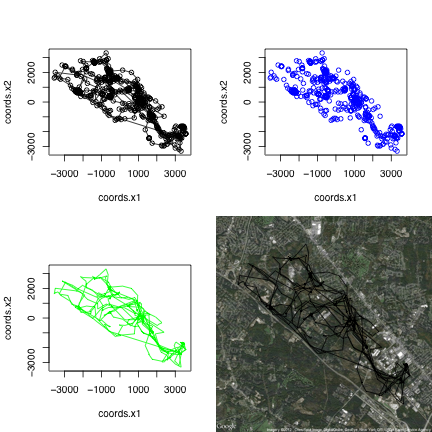
\includegraphics{move-fig1}
\end{center}
\caption{Plotting the UD (left) and adding the track as a line (center) or as points (right)}
\label{fig:two}
\end{figure}

To plot contour lines from the raster, use the \fct{contour} function and set the percentage levels that you want to print. With \texttt{add=TRUE} you can add the contour to a previous plot (see Figure \ref{fig:three}). \\

\begin{figure}
\begin{center}
\begin{Schunk}
\begin{Sinput}
> plot(ricky_dbbmm, xlab="location_long", ylab="location_lat")
> contour(ricky_dbbmm, levels=c(.5, .95), col=c(6,2), add=TRUE, lwd=2)
\end{Sinput}
\end{Schunk}
\includegraphics{move-contour}
\end{center}
\caption{Plotting the 95\% and 50\% contour lines on top of the UD.}
\label{fig:three}
\end{figure}

\fct{raster}              : returns the information of the stored raster\\
\fct{outerProbability}    : calculates the probabilities of the UD at the border of the raster\\


\subsection{Calculating UD area size}
To determine the area size of the UD, we need to calculate the contour raster from the UD raster. This means, that each raster has not longer its original value but the value of the contour it belongs to. A cell with a very high value in the UD raster will have a very low value in the contour raster. We will use the \texttt{getVolumeUD()} function to calculate the contour raster and then create a new raster that includes only the cells that belong to the 95\% contour. Cells that belong to the contour will get the value 1 while the others get 0. In the last step we can just sum the values of the raster. The area is the number of cells (which we just calculated) multiplied by the actual size of the raster cells. 

\begin{Schunk}
\begin{Sinput}
> ricky_cont <- getVolumeUD(ricky_dbbmm)
> ricky_cont <- ricky_cont<=.95
> area <- sum(values(ricky_cont))
> area
\end{Sinput}
\begin{Soutput}
[1] 714
\end{Soutput}
\end{Schunk}

\subsection{Storing and loading objects}
If one or more objects should be stored and loaded at another time into R, there is an easy way to save them. The \fct{save} function saves all listed objects from the workspace (in the example below it is only ricky\_dbbmm). The file format is \texttt{RData}. More than one variable or the whole workspace can be stored in a \texttt{RData} file. Complicated calculations (e.g. Brownian bridges), can be calculated once and then stored. \\
\texttt{RData} files can be loaded using the \fct{load} function. It loads all objects from the file again into the workspace. In the following example we save the object \texttt{ricky\_dbbmm} as \texttt{test.RData}, remove the object (it does not appear any more in the workspace), and load it again.

\begin{Schunk}
\begin{Sinput}
> save(x=ricky_dbbmm, file="~/Desktop/test.RData")
> rm(ricky_dbbmm)
> load(file="~/Desktop/test.RData")
\end{Sinput}
\end{Schunk}


\subsection{Store a track as a KML file}
\class{Move} objects can also be saved as KML (keyhole markup language) files. KML files can easily be loaded into GoogleEarth and GoogleMaps. For this the \texttt{plotKML} package is needed. Once installed the \fct{kml} function creates a file with the ending \texttt{.kml} and the name of the object. The kml file is then stored in the current working directory. \\
The following code creates the file \texttt{leroy.kml} from the \class{Move} object named \texttt{leroy}. If GoogleEarth is installed, a double click on that file opens the locations of the track in GoogleEarth.

\begin{Schunk}
\begin{Sinput}
> #install.packages('plotKML')
> require(plotKML)
> kml(leroy)
\end{Sinput}
\end{Schunk}


%\newpage

\section{Home Range Bootstrap using Minimum Convex Polygons}
The move package includes a method to calculate minimum convex polygons (MCP) using \fct{hrBootstrap}. A minimum convex polygon describes an area that is formed by the points of a track. The convex is because no line that connects two points within this polygon crosses the border of the polygon. \\
We implemented this method to calculate MCPs from the \texttt{adehabitatHR} package (more information) using a bootstrap method. This means that the area size of the MCP is calculated with an (exponentially) increasing number of coordinates. The MCP size continues to increase until it reaches a plateau. \\
Because the function takes random coordinates to calculate the MCP, every calculation is repeated 100 times by default. For every number of coordinates the quantiles are calculated and plotted in a line diagram. A black horizontal line indicates the real MCP size (calculated with all coordinates).

\begin{figure}
\begin{center}
\begin{Schunk}
\begin{Sinput}
> hrBootstrap(x=leroy, rep=100, unin='km', unout='km2')
\end{Sinput}
\end{Schunk}
\includegraphics{move-hrBootstrap}
\end{center}
\caption{The returned plot forms the \fct{hrBootstrap} for a track with 100 repetitions.}
\label{fig:four}
\end{figure}



\end{document}
